%-----------------------------------------------------------------
%	BASIC DOCUMENT LAYOUT
%-----------------------------------------------------------------
\documentclass[paper=a4, fontsize=12pt, twoside=semi, abstracton, listof=totoc, toc=left]{scrartcl}
\usepackage[T1]{fontenc}
\usepackage[utf8]{inputenc}
\usepackage{lmodern}
\usepackage{slantsc}
\usepackage{microtype}
\usepackage[british]{babel}
% \usepackage[backend=bibtex, style=phys, sorting=none, citestyle=authoryear, maxbibnames=3, maxcitenames=2]{biblatex}
\usepackage[backend=bibtex, style=trad-abbrv, sorting=none, maxbibnames=3, maxcitenames=2]{biblatex}
\addbibresource{bibliography.bib}
% \bibliographystyle{apalike}
\makeatletter
	\def\blx@maxline{77}
\makeatother

% Sectioning layout
\addtokomafont{sectioning}{\normalfont\scshape}
\usepackage{tocstyle}
\usetocstyle{standard}
\renewcommand*\descriptionlabel[1]{\hspace\labelsep\normalfont\bfseries{#1}}
\usepackage[titletoc]{appendix}

% Empty pages
\usepackage{etoolbox}
% \pretocmd{\toc}{\cleardoubleevenemptypage}{}{}
% \pretocmd{\section}{\cleardoubleevenemptypage}{}{}
\pretocmd{\part}{\cleardoubleevenemptypage\thispagestyle{empty}}{}{}
\renewcommand\partheadstartvskip{\clearpage\null\vfil}
\renewcommand\partheadmidvskip{\par\nobreak\vskip 20pt\thispagestyle{empty}}

% Paragraph indentation behaviour
\setlength{\parindent}{0pt}
\setlength{\parskip}{0.3\baselineskip plus2pt minus2pt}
\newcommand{\sk}{\medskip\noindent}

% Fancy header and footer
\usepackage{fancyhdr}
\pagestyle{fancyplain}
\fancyhead[LO]{\thepage}
\fancyhead[CO]{}
\fancyhead[RO]{\nouppercase{\mytitle}}
\fancyhead[LE]{\nouppercase{\rightmark}}
% \fancyhead[LE]{\nouppercase{\leftmark}}
\fancyhead[CE]{}
\fancyhead[RE]{\thepage}
\fancyfoot{}
\renewcommand{\headrulewidth}{0.3pt}
\renewcommand{\footrulewidth}{0pt}
\setlength{\headheight}{13.6pt}

%-----------------------------------------------------------------
%	MATHS AND SCIENCE
%-----------------------------------------------------------------
\usepackage{amsmath,amsfonts,amsthm,amssymb}
\usepackage{xfrac}
\usepackage[a]{esvect}
\usepackage{chemformula}
\usepackage{graphicx}
	\graphicspath{{images/}}

\usepackage[arrowdel]{physics}
	\renewcommand{\vnabla}{\vec{\nabla}}
	% \renewcommand{\vectorbold}[1]{\boldsymbol{#1}}
	% \renewcommand{\vectorarrow}[1]{\vec{\boldsymbol{#1}}}
	% \renewcommand{\vectorunit}[1]{\hat{\boldsymbol{#1}}}
	\renewcommand{\vectorarrow}[1]{\vec{#1}}
	\renewcommand{\vectorunit}[1]{\hat{#1}}
	\renewcommand*{\grad}[1]{\vnabla #1}
	\renewcommand*{\div}[1]{\vnabla \vdot \va{#1}}
	\renewcommand*{\curl}[1]{\vnabla \cp \va{#1}}
	\let\rot\curl

% SI units
\usepackage[separate-uncertainty=true]{siunitx}
% \sisetup{range-phrase = \text{--}, range-units = brackets}
\sisetup{range-phrase = \text{--}, range-units = single}
\DeclareSIPrePower\quartic{4}
	%\DeclareSIUnit\micron{\micro\metre}

% Smaller trig functions
\newcommand{\Sin}{\trigbraces{\operatorname{s}}}
\newcommand{\Cos}{\trigbraces{\operatorname{c}}}
\newcommand{\Tan}{\trigbraces{\operatorname{t}}}

% Operator-style notation for matrices
\newcommand*{\mat}[1]{\hat{#1}}

% Matrices in (A|B) form via [c|c] option
\makeatletter
\renewcommand*\env@matrix[1][*\c@MaxMatrixCols c]{%
  \hskip -\arraycolsep
  \let\@ifnextchar\new@ifnextchar
  \array{#1}}
\makeatother

% Shorter \mathcal and \mathbb
\newcommand*{\mc}[1]{\mathcal{#1}}
\newcommand*{\mbb}[1]{\mathbb{#1}}

% Shorter ^\ast and ^\dagger
\newcommand*{\sast}{^{\star}{}}
\newcommand*{\sdag}{^{\dagger}{}}

% Blackboard bold identity
\usepackage{bbm}
\newcommand*{\bbid}{\mathbbm{1}}

% Shorter displaystyle
\newcommand*{\dsp}{\displaystyle}

% Inexact differential
\newcommand{\dbar}{\mathchar'26\mkern-12mu\mathrm{d}}
\newcommand{\indd}[1]{\dbar{#1}}

% Arrows with text and cancels for developments
\newcommand{\tikzmark}[1]{\tikz[overlay,remember picture] \node (#1) {};}
\tikzset{square arrow/.style={to path={-- ++(0,-.25) -| (\tikztotarget)}}}
\usepackage{cancel}

\newcommand*\acr[1]{\textscale{.85}{#1}}

%-----------------------------------------------------------------
%	OTHER PACKAGES
%-----------------------------------------------------------------
\usepackage{environ}

%Left numbered equations
\makeatletter
	\NewEnviron{Lalign}{\tagsleft@true\begin{align}\BODY\end{align}}
\makeatother

% Plots and graphics
\usepackage{pgfplots}
\usepackage{tikz}
\usepackage{color}
	\makeatletter
		\color{black}
		\let\default@color\current@color
	\makeatother

% Richer enumerate, figure, and table support
\usepackage{enumerate}
\usepackage[shortlabels]{enumitem}
\usepackage{float}
\usepackage{tabularx}
\usepackage{booktabs}
	%\setlength{\intextsep}{8pt}
% \numberwithin{equation}{section}
% \numberwithin{figure}{section}
% \numberwithin{table}{section}
% \counterwithin{lstlisting}{section}

% No indentation after certain environments
\makeatletter
\newcommand*\NoIndentAfterEnv[1]{%
	\AfterEndEnvironment{#1}{\par\@afterindentfalse\@afterheading}}
\makeatother
%\NoIndentAfterEnv{thm}
\NoIndentAfterEnv{defi}
\NoIndentAfterEnv{example}
\NoIndentAfterEnv{table}

% Misc packages
\usepackage{ccicons}
\usepackage{lipsum}
\usepackage{todonotes}
\usepackage{array}
\usepackage{multirow}

% Print DOI only if there's no URL
\renewbibmacro*{doi+eprint+url}{%
  \iftoggle{bbx:doi}
    {\iffieldundef{url}{\printfield{doi}}{}}
    {}%
  \newunit\newblock
  \iftoggle{bbx:eprint}
    {\usebibmacro{eprint}}
    {}%
  \newunit\newblock
  \iftoggle{bbx:url}
    {\usebibmacro{url+urldate}}
    {}}

%-----------------------------------------------------------------
%	SYNTAX HIGHLIGHTING
%-----------------------------------------------------------------
\usepackage[formats]{listings}
\usepackage{relsize}
\usepackage{chngcntr}

\renewcommand{\lstlistingname}{Snippet}
\renewcommand{\lstlistlistingname}{List of snippets}

\lstloadlanguages{python,bash}
\lstdefinelanguage{Renhanced}[]{R}{%
	morekeywords={acf,ar,arima,arima.sim,colMeans,colSums,is.na,is.null,%
	mapply,ms,na.rm,nlmin,replicate,row.names,rowMeans,rowSums,seasonal,%
	sys.time,system.time,ts.plot,which.max,which.min,%
	rename,mutate,unite,select,filter,left_join,group_by,dplyr::select,%
	ggplot,aes,geom_line,geom_hline,geom_point,geom_path,geom_errorbar,%
	geom_abline,geom_smooth%
	geom_cartogram,coord_proj,scale_x_longitude, scale_y_latitude,%
	labs,guides,annotate,theme,rowwise,%
	scale_linetype_manual,scale_colour_manual,scale_x_log10,scale_y_log10,%
	attr,paste,paste0,bind_rows,str_trim,as.numeric,as.dataframe,data.frame},
	deletekeywords={c,range,step},
	alsoletter={.,_,::},
	otherkeywords = {!,!=,~,\$,*,\&,\%/\%,\%*\%,\%\%,\%>\%,<-,<<-,\% in \%}
	}

\newcommand*{\inline}{\lstinline[basicstyle=\normalsize\ttfamily]}


\lstset{language=python,
		frame=tb,
		% captionpos=b,
		tabsize=2,
		% showtabs=true,
		breaklines=true,
		breakatwhitespace=true,
		basicstyle=\smaller\ttfamily,
		numbers=left,
		numberstyle=\tiny,
		numbersep=7.5pt,
		% commentstyle=\textsl,
		xleftmargin=3ex}
\lstset{escapeinside={(*}{*)}}   % for (*\ref{ }*) inside lstlistings (Scode)

\lstdefinestyle{output}{
	language=,
	% showtabs=true,
	% showspaces=true,
	numbers=none,
	frame=tblr,
	% columns=fullflexible,
	% backgroundcolor=\color{blue!10},
	numbers=none,
	xleftmargin=3ex}

\expandafter\patchcmd\csname \string\lstinline\endcsname{%
	\leavevmode
	\bgroup
}{%
	\leavevmode
	\ifmmode\hbox\fi
	\bgroup
}{}{%
	\typeout{Patching of \string\lstinline\space failed!}%
}
%% end of patch

%-----------------------------------------------------------------
%	THEOREMS
%-----------------------------------------------------------------
\usepackage{thmtools}

% Theroems layout
\declaretheoremstyle[
	spaceabove=6pt, spacebelow=6pt,
	headfont=\normalfont,
	notefont=\mdseries, notebraces={(}{)},
	bodyfont=\small,
	postheadspace=1em,
]{small}

\declaretheorem[style=plain,name=Theorem,qed=$\square$,numberwithin=section]{thm}
\declaretheorem[style=plain,name=Corollary,qed=$\square$,sibling=thm]{cor}
\declaretheorem[style=plain,name=Lemma,qed=$\square$,sibling=thm]{lem}
\declaretheorem[style=definition,name=Definition,qed=$\blacksquare$,numberwithin=section]{defi}
\declaretheorem[style=definition,name=Example,qed=$\blacktriangle$,numberwithin=section]{example}
\declaretheorem[style=small,name=Proof,numbered=no,qed=$\square$]{sproof}

%-----------------------------------------------------------------
%	ELA MOTHERFUCKING GEMINADA
%-----------------------------------------------------------------
\def\xgem{%
	\ifmmode
		\csname normal@char\string"\endcsname l%
	\else
		\leftllkern=0pt\rightllkern=0pt\raiselldim=0pt
		\setbox0\hbox{l}\setbox1\hbox{l\/}\setbox2\hbox{.}%
		\advance\raiselldim by \the\fontdimen5\the\font
		\advance\raiselldim by -\ht2
		\leftllkern=-.25\wd0%
		\advance\leftllkern by \wd1
		\advance\leftllkern by -\wd0
		\rightllkern=-.25\wd0%
		\advance\rightllkern by -\wd1
		\advance\rightllkern by \wd0
		\allowhyphens\discretionary{-}{}%
		{\kern\leftllkern\raise\raiselldim\hbox{.}%
			\kern\rightllkern}\allowhyphens
	\fi
}
\def\Xgem{%
	\ifmmode
		\csname normal@char\string"\endcsname L%
	\else
		\leftllkern=0pt\rightllkern=0pt\raiselldim=0pt
		\setbox0\hbox{L}\setbox1\hbox{L\/}\setbox2\hbox{.}%
		\advance\raiselldim by .5\ht0
		\advance\raiselldim by -.5\ht2
		\leftllkern=-.125\wd0%
		\advance\leftllkern by \wd1
		\advance\leftllkern by -\wd0
		\rightllkern=-\wd0%
		\divide\rightllkern by 6
		\advance\rightllkern by -\wd1
		\advance\rightllkern by \wd0
		\allowhyphens\discretionary{-}{}%
		{\kern\leftllkern\raise\raiselldim\hbox{.}%
			\kern\rightllkern}\allowhyphens
	\fi
}

\expandafter\let\expandafter\saveperiodcentered
	\csname T1\string\textperiodcentered \endcsname

\DeclareTextCommand{\textperiodcentered}{T1}[1]{%
	\ifnum\spacefactor=998
		\Xgem
	\else
		\xgem
	\fi#1}

%-----------------------------------------------------------------
%	DEDICATION ENVIRONMENT
%-----------------------------------------------------------------

\newenvironment{mydedication}
	{\clearpage           % we want a new page
	\thispagestyle{empty}% no header and footer
	\vspace*{\stretch{1}}% some space at the top
	\itshape             % the text is in italics
	\raggedleft          % flush to the right margin
	}
	{\par % end the paragraph
	\vspace{\stretch{3}} % space at bottom is three times that at the top
	\clearpage           % finish off the page
	}

%-----------------------------------------------------------------
%	PDF INFO AND HYPERREF
%-----------------------------------------------------------------
\usepackage{hyperref}
\hypersetup{colorlinks, citecolor=black, filecolor=black, linkcolor=black, urlcolor=black}
\usepackage{cleveref}
	\crefname{section}{\S}{\SS}
	\Crefname{section}{\S}{\SS}
	\crefname{listing}{snippet}{}

\newcommand*{\mytitle}{N Queens Problem}
\newcommand*{\mysubtitle}{An implementation using Genetic Algorithms and Python}
\newcommand*{\myauthor}{Alfredo Hernández}
% \newcommand*{\mysupervisor}{J. Minguillón}
% \newcommand*{\mytutor}{}
\newcommand*{\myuni}{Universitat Autònoma de Barcelona}
\newcommand*{\mydate}{30th November 2017}
% \newcommand*{\mydate}{10th December} # Deadline

\pdfstringdefDisableCommands{\def\and{and }}

\usepackage{hyperxmp}
\hypersetup{pdfauthor={\myauthor}, pdftitle={\mytitle: \mysubtitle}}

%-----------------------------------------------------------------
%	TITLE SECTION AND DOCUMENT BEGINNING
%-----------------------------------------------------------------
\newcommand{\horrule}[1]{\rule{\linewidth}{#1}}
\title{
	\normalfont
	\small \scshape{\myuni} \\ [25pt]
	\horrule{0.5pt} \\ [0.4cm]
	\huge \mytitle \\
	\Large \scshape{\mysubtitle} \\
	\horrule{2pt} \\ [0.5cm]
}
\author{\myauthor }
% \\ \footnotesize Supervised by: \mysupervisor \\ \footnotesize Academic tutor: \mytutor}
\date{\mydate}

\begin{document}

\clearpage\maketitle
\thispagestyle{empty}
\addtocounter{page}{-1}

%-----------------------------------------------------------------
%	DEDICATION
%-----------------------------------------------------------------
% \begin{mydedication}
% 	Dedicated to RMT, Val \& the Brotherhood
% \end{mydedication}

%-----------------------------------------------------------------
%	DOCUMENT BODY
%-----------------------------------------------------------------
\cleardoubleevenemptypage
% %-----------------------------------------------------------------
%	ABSTRACT
%	!TEX root = ./../main.tex
%-----------------------------------------------------------------
\cleardoubleevenemptypage
\thispagestyle{empty}
\phantomsection
\addcontentsline{toc}{section}{Abstract}
\begin{abstract}
	Crime Data Analysis is an already established yet flourishing topic in the United States. Despite that, there is no public user-friendly global data hub to visualise crime statistics across the US territory. The goal of this work is to create dynamic time series visualisations of the evolution of crime in different cities of the US. The mission of this work is to develop visualisation tools in order to further ease the access to already open data. Using the R language we gather open databases of different cities and unify the data into a single standard format, leading to straightforward comparative methods. We would like to see whether or not crime statistics change significantly throughout the different regions of the US and if there are clear trends that help us identify geographical differences in the American society. Last but not least, we would like to look for temporal patterns that could be identified with major global or local events.
\end{abstract}


\pdfbookmark[1]{\contentsname}{toc}
\tableofcontents

%-----------------------------------------------------------------
%	TOOLS AND DATA
%	!TEX root = ./../main.tex
%-----------------------------------------------------------------
\section[The N Queens Problem]{The $N$ Queens Problem}\label{sec:problem}\nocite{Pearl1984}
This problem consists on placing $N$ queens on a $N \times N$ chessboard so that no queen can attack another. In the usual fashion, an attack is defined when two or more queens are in the same row, column, or diagonal (as depicted in figure \ref{fig:4queens}). We will expand on how to compute if a queen attacks another in \cref{sec:fitness}.

\begin{figure}[H]
	\centering
	\includegraphics[height=0.18\textwidth]{4queens}
	\caption{Example of a queen attacking another queen on a $4 \times 4$ board}
	\label{fig:4queens}
\end{figure}

The problem can be quite expensive from a computational point of view, as there are $N^{N}$ possible arrangements of $N$ queens on an $N \times N$ board, but only a small amount of solutions (relative to the total possible arrangements). It is possible, however, to use shortcuts that reduce computational requirements of brute-force techniques.

\subsection{Computational representation}\label{sec:representation}
Given the nature of this problem, we can program our algorithm to work with queens so that no queen shares the same row or column. The simplest way is to think of each board as an array of non-repeated consecutive numbers, where the index represents the row, and the number itself is the column; this is called \emph{Permutation Representation}. For instance, the board in figure \ref{fig:4queens} would be represented as
\begin{align}
	\inline{[1 2 0 3]}.
\end{align}

This consideration alone makes the complexity of a brute-force algorithm much simpler, as now we only have $N!$ possible permutations of $N$ queens on an $N \times N$ board (we will expand on this later).

%-----------------------------------------------------------------
\subsection{Solutions of the problem}

Table \ref{tab:all-sols} summarises the number of solutions for the $N$ Queens Problem, both fundamental and all (or non-fundamental) solutions, where fundamental solutions are those that exclude mirrored images as well as rotations of a solution.

There is currently no known formula for the exact number of solutions, or even for its asymptotic behaviour for larger values of $N$.
\begin{table}[H]
	\centering
	\begin{tabular}{r | ccccccccccc}
		\toprule
		\toprule
		$N$         & 1 & 2 & 3 & 4 & 5 & 6 & 7 & 8 & 9 & 10 & ... \\
		\midrule
		fundamental & 1 & 0 & 0 & 1 & 2 & 1 & 6 & 12 & 46 & 92 & ... \\
		all         & 1 & 0 & 0 & 2 & 10 & 4 & 40 & 92 & 352 & 724 & ... \\
		\bottomrule
	\end{tabular}
	\caption{List of solutions for the $N$ Queens Problem}
	\label{tab:all-sols}
\end{table}

All non-fundamental solutions up to $N = 10$ can be easily obtained using the script \inline{brute-queens.py}. We will not discuss the details of the implementation, for it is a really simple algorithm, and brute-force methods are not the main focus of this text.

As an illustration, in figure \ref{fig:4queens-sols} we depict the only two non-fundamental solutions for $N = 4$. It is worth to notice that the two solutions are the same fundamental solution, as they are the mirrored image of each other.

\begin{figure}[H]
	\centering
	\includegraphics[height=0.18\textwidth]{4queens-sols}
	\caption{The two non-fundamental solutions of the 4 Queens Problem}
	\label{fig:4queens-sols}
\end{figure}

In figure \ref{fig:queens-sols} we compare the complexity of using an algorithm that calculates all possible arrangements and another that only calculates all the possible permutations against the amount of non-fundamental solutions for the $N$ Queens Problem.
\begin{figure}[H]
	\centering
	\includegraphics[width=0.95\textwidth]{queens-sols}
	\caption{Comparison of brute-force complexity for the $N$ Queens Problem}
	\label{fig:queens-sols}
\end{figure}

%-----------------------------------------------------------------
\subsection{Role of metaheuristics}
One may think that using only permutations gives us a good enough brute-force method to solve this problem. This may be true for small values of $N$, but $N > 10$ presents quite a computational barrier in terms of memory requirements. Using $N = 11$ requires calculating $11! = \num{39916800}$ different permutations; this means using $\sim \SI{3.5}{GB}$ of RAM\footnote{On a 64-bit platform (8 bits per integer).} just to store the numbers on the boards (the boards' structure would be another thing altogether).

It is for this reason that heuristics are used to solve this kind of problem, as they can be used to speed up the process of finding a solution. In particular, we will solve the $N$ Queens Problem using a Genetic Algorithm, a metaheuristic inspired by the process of natural selection that belongs to the larger class of evolutionary algorithms. We will discuss this implementation in \cref{sec:implementation}.




%-----------------------------------------------------------------
%	RESULTS
%	!TEX root = ./../main.tex
%-----------------------------------------------------------------
\section{Implementation with a Genetic Algorithm}\label{sec:implementation}\nocite{Sean2010}
\subsection{Methodology of a Genetic Algorithm}\label{sec:genetic-alg-structure}
The Genetic Algorithm was invented by John Holland at the University of Michigan in the 1970s. This evolutionary algorithm consists on iterating through fitness assessment, recombination, and population reassembly.

In the recombination process, we select two parents from the original population, cross them over with one another, and mutate the results. The children are then reassembled into the original population (the way to do this varies from author to author).

\bigskip
\textcite{Zapfel2010} go into great detail on how each component of the algorithm affects the solution of the problem. In figure \ref{fig:structure} we can see a simple diagram on how the Genetic Algorithm is structured and how each operation depends on the specific problem one wants to tackle.
\begin{figure}[H]
	\centering
	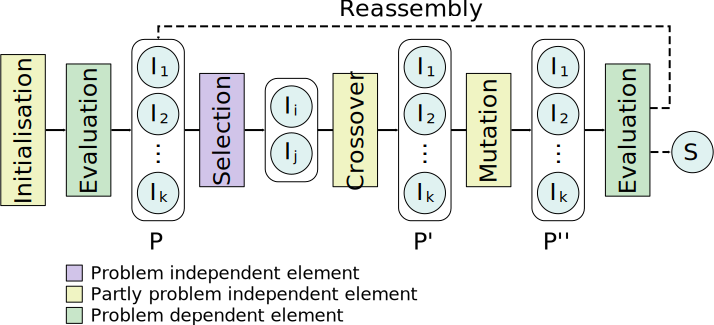
\includegraphics[width=0.8\textwidth]{genetic-algorithm}
	\caption{Structure of a Genetic Algorithm}
	\label{fig:structure}
\end{figure}

One might wonder why initialisation, crossover, and mutation are marked as partly problem dependent here. The reason is that in Genetic Algorithms, different encodings can be used to represent individuals. By using simple or generic encodings, like binary or permutation, one can use standard genetic operators for crossover and mutation. Hence these operators are referred to as partly problem dependent. %The main advantage is the applicability of generic crossover and mutation operators, i.e. no problem specific operators must be developed.

%-----------------------------------------------------------------
\subsection{Computational structure of the program}\label{sec:program}
First of all, we need to decide the programming language we will use to implement the Genetic Algorithm. I decided to use Python 3, as I am more experienced with it, and because it would allow me to tweak the program and play with the different parameters without focusing too much on the technical side of things.

One of the main advantages of using an object-oriented programming language like Python is the ability to use classes to group each individual with its properties (sequence and fitness) in an organised and straightforward way. In \cref{sn:class} we can see the \inline{BoardPermutation} class we will use to store each one of the individuals or \inline{board}s.

\begin{lstlisting}[label=sn:class, caption=Definition of the \inline{BoardPermutation} class]
class BoardPermutation:
	def __init__(self):
		self.sequence = None
		self.fitness = None
	def set_sequence(self, val):
		self.sequence = val
	def set_fitness(self, fitness):
		self.fitness = fitness
	def get_attr(self):
		return { 'sequence' : sequence, 'fitness' : fitness }
\end{lstlisting}

In the following sections we will see how \inline{sequence} and \inline{fitness} are defined.

%-----------------------------------------------------------------
\subsection{Initialisation of the population}\label{sec:init}

Now that we know the computational structure of the individuals, we can work out a function to generate each of the individuals that constitute the initial population. In \cref{sn:generate_chromosome} we can see how we define our \inline{generate_chromosome()} function. What the function does is generate an ordered array from \inline{0} to \inline{N_QUEENS} (as in \inline{[0 1 2 3 ... N_QUEENS]}), and then shuffle the elements to create different permutations. For the sake of academic rigour, as is usual with Genetic Algorithms, we call each individual a chromosome.

\begin{lstlisting}[label=sn:generate_chromosome, caption=Function to generate a single individual]
def generate_chromosome():
	# Randomly generates a sequence of board states.
	init_distribution = np.arange(N_QUEENS)
	np.random.shuffle(init_distribution)
	return init_distribution
\end{lstlisting}

Notice that we are using Python's \inline{numpy} library, which makes our program run almost as fast\footnote{Provided we know how to make an efficient program (which is probably not the case).} as if it used native C. %This is, as is usual with powerful and fast libraries, because \inline{numpy} is written in C.

All we have to do now is to generate the initial population. The implementation is straightforward: we create a list of \inline{population_size} objects of class \inline{BoardPermutation}. Then all we need to do is to set the sequence and the fitness of each board using the \inline{generate_chromosome()} and \inline{assess_fitness()} functions, respectively. This is clearly illustrated in \cref{sn:generate_population}.

\begin{lstlisting}[label=sn:generate_population, caption=Population initialization function]
def generate_population(population_size = 100):
	# Create the different boards
	population = [BoardPermutation() for i in range(population_size)]
	for i in range(population_size):
		population[i].set_sequence(generate_chromosome())
		population[i].set_fitness(assess_fitness(population[i].sequence))
	return population
\end{lstlisting}

%-----------------------------------------------------------------
\subsection{Evaluation: fitness function}\label{sec:fitness}

The evaluation function determines the quality of a candidate solution. In metaheuristics this is usually called fitness function. The fitness value of a proposed solution is needed for the selection process and eventually finding the final solution of our problem.

As we mentioned before, the assessment of the fitness of a solution is a problem dependent element. In \cref{sec:representation} and \cref{sec:init} we discussed how we only worked with permutations of an array of non-repeated consecutive numbers. This eases the calculation of the fitness quite a bit.

Since the queens are by definition in different rows and columns, we only have to check if a queen attacks another one diagonally. We could do this by iterating on the diagonal cells of any given queen and check if there is a queen in any of the cells, but this is a bit complex to program. We found that the easiest way to check if two queens attack each other is to check if
\begin{align}
	\abs{ x_{i} - x_{j} } = \abs{ y_{i} - y_{j} } ,
\end{align}
that is, when the two queens' vertices define a square, as depicted in figure \ref{fig:4queens-attack}.

\begin{figure}[H]
	\centering
	\includegraphics[height=0.18\textwidth]{4queens-attack}
	\caption{Example of a queen attacking another queen}
	\label{fig:4queens-attack}
\end{figure}

In \cref{sn:assess_fitness} we can see our implementation of the fitness function. In it we count the amount of clashes produced in any given board, then we return \inline{MAX_FIT - clashes}. In this problem, \inline{MAX_FIT} is $N (N-1)$; the reason behind this is really simple. We can think of the queens as a set of $N$ vertices; in a $K_{N}$ graph, the amount of edges is $v (v-1)/ 2$, where edges connect queens that do not clash with one another. The reason behind the $\times 2$ factor is that we count clashes twice in our loop ($Q_{i}$ attacks $Q_{j}$ and $Q_{j}$ attacks $Q_{i}$); this does not matter as long as our fitness function is well defined and behaves in a controlled way.

\begin{lstlisting}[label=sn:assess_fitness, caption=Fitness function]
def assess_fitness(chromosome = None):
	clashes = 0
	# Calculate diagonal clashes
	for i in range(len(chromosome)):
		for j in range(len(chromosome)):
			if ( i != j):
				dx = abs(i-j)
				dy = abs(chromosome[i] - chromosome[j])
				if(dx == dy):
					clashes += 1
	return (MAX_FIT - clashes)
\end{lstlisting}

%-----------------------------------------------------------------
\subsection{Reassembly of the population}\nocite{Zapfel2010}

Before we explain the recombination process, we need to define how the reassembly of the population will be done in our program. This is very important, because it will directly define the way we implement the parent selection and crossover process.

The reassembly process consists on replacing old individuals with new ones. There are several replacement strategies, the following being the most popular:
\begin{itemize}
	\item Generational Replacement.
	\item Steady-State Replacement.
\end{itemize}

In Generational Replacement the new generation supersedes the old generation. But this replacement scheme has a big disadvantage. If one replaces the whole generation the risk of dismissing a very promising solution is high.

In contrast, Steady-State Replacement consists on dynamically replacing old individuals by new ones. But whether only a single individual or multiple individuals are replaced,  so one must define which individuals are replaced (worst, random, parents, ...)

\bigskip
In our implementation we will perform a Steady-State Replacement of the parents.

%-----------------------------------------------------------------
\subsection{Recombination process}\label{sec:recombination}
This is probably the most important part of the whole Genetic Algorithm. This is where we need to choose if we want to focus on exploitation (corresponding to intensification) or exploration (corresponding to diversification). This is not an easy task, because in an ideal scenario, we want the balance between both; as \textcite{Stutzle1999} puts it
\begin{quotation}
	\emph{A metaheuristic will be successful on a given optimization problem if it can provide a balance between the exploitation of the accumulated search experience and the exploration of the search space to identify regions with high quality solution in a problem specific, near optimal way.}
\end{quotation}

Not only that, but using a population of permutation individuals has a trade-off of having an easier fitness function: the crossover function has to be modified to avoid getting an invalid children when recombining two parents (e.g., \inline{[1 1 0 3]}). Although most texts deal with crossovers in the most generalised manner, some do make this distinction and tweak the classical algorithms to impede such children, such as \textcite{Gendreau2010}, and \textcite{Goldberg1989}. The same is true for the mutation function, although the workaround is fairly straightforward.

%-----------------------------------------------------------------
\subsubsection*{Parent selection}%\nocite{Gendreau2010}
As mentioned before, the parent selection is trivial, as it does not depend on the structure of our individuals; the only important parameter is their fitness.

The usual selection methods involve ranking in some fashion all individuals by their fitness. The most widely used method is the Fitness-Proportionate Selection, also known as Roulette Selection. This method is discussed in detail by \textcite{Sean2010} and \textcite{Gendreau2010}; in short it selects individuals with higher fitness more often (this involves defining a selection pressure, or a survival function).

The method we will use, however, is the Tournament Selection. In this selection method a set of $\tau$ (this is called the Tournament Size) chromosomes are chosen and compared, the best one being selected for parenthood. Our implementation can be seen in \cref{sn:tournament}.

\begin{lstlisting}[label=sn:tournament, caption=Parent selection using a Tournament Selection]
def get_parent(population = None):
	# Get parent using a Tournament Selection algorithm
	best_board = random.randint(0, len(population) - 1)
	for i in range(1,TOURN_SIZE):
		next_board = random.randint(0, len(population) - 1)
		if ( population[next_board].fitness > population[best_board].fitness ):
			best_board = next_board
	return best_board
\end{lstlisting}

Using a Tournament Selection over a Fitness-Proportionate Selection has quite a number of advantages. First of all, the Tournament Selection can deal with situations where there is no formal objective fitness function (needed to define the selection pressure), as it is not sensitive to how the fitness is defined; it only needs the fitness value itself. Second, it is not a complex method, leading to very fast computational times. Last but not least, it can be finely tuned to our liking; allowing us to be more exploratory or exploitatory.

In the Genetic Algorithm, the most popular setting is $\tau = 2$; this approach has similar properties to Fitness-Proportionate Selection. This value for the Tournament Size leads to a fairly exploratory algorithm, but using bigger values makes the algorithm too exploitatory, which can lead to very slow (or very fast, depending on the initial population\footnote{This can be understood in terms of Lyapunov's instability principle.}) convergence.

In \cref{sec:parameter-control} we will discuss in more detail how we will choose the optimal value for $\tau$ as well as the other parameters involved in the Genetic Algorithm.

%-----------------------------------------------------------------
\subsubsection*{Crossover process}\nocite{Goldberg1989}

Under a standard Two-Point Crossover, two parents are aligned and two crossing points are picked uniformly at random. These two points define a matching region, which are swapped between the two parents, giving place to two children:

\begin{align}
	\mqty{
	P_{1}: & \inline{[ 0 4 | 2 3 1 | 5 ]} \\
	P_{2}: & \inline{[ 5 0 | 2 1 4 | 3 ]}
	}
	\, \mapsto \,
	\mqty{
	P_{1}': & \inline{[ 0 4 | 2 1 4 | 5 ]} \\
	P_{2}': & \inline{[ 5 0 | 2 3 1 | 3 ]}
	 }.
\end{align}

The first thing we notice is that this simple crossover has led to two invalid individuals under our Permutation Representation, just as we warned in \cref{sec:recombination}. This will surely be the case for most crossovers. So let us find a better suited crossover function for the problem in our hands.

The Partially-Matched Crossover, or PMX, tries to solve this problem. Its philosophy is very similar to that of the Two-Point Crossover: two points are randomly selected to define a matching region. The difference is that the matching region defines a position-by-position interchange mapping. Let us see this with an example:

\begin{align}
\begin{gathered}
	\mqty{
	P_{1}: & \inline{[ 0 4 | 2 3 1 | 5 ]} \\
	P_{2}: & \inline{[ 5 0 | 2 1 4 | 3 ]}
	}
	\, \mapsto \,
	\mqty{
	P_{1}': & \inline{[ 0 1 2 4 3 5 ]} \\
	P_{2}': & \inline{[ 5 0 2 3 1 4 ]}
	 },
\end{gathered}
\end{align}
where $\qty{ 2 \leftrightarrow 2, 3 \leftrightarrow 1, 1 \leftrightarrow 4 }$ is our set of interchange mappings.

Even so, not everything is perfect with this crossover: in some situations one may end up with a set of interchange mappings that contain a number more than once (just as the example above). In my opinion\footnote{I am sure the PMX works just fine, but I am not particularly fond of it from a philosophical and programming point of view.}, this crossover has an unclear order of operations (in the example above we did the interchange mappings from left to right, but we could have done them in any order) and inevitably leads to redundant calculations.

\bigskip
\textcite{Goldberg1989} explores several crossover algorithms similar to the PMX that can be easily applied to problems with Permutation Representation. In particular, we will focus on the Ordered Crossover, or OX.

The OX starts in a similar fashion as the PMX: two points are randomly selected to define a matching region. Like PMX, each string maps to constituents of the matching section of its mate. Instead of using point-by-point interchange mapping, OX uses a sliding motion to fill the holes left by transferring the mapped positions. For example when parent $P_{2}$ maps to parent $P_{1}$; queens 2, 3, and 1 will leave holes (marked by an \inline{H}) in the board:
\begin{align}
	\mqty{ P_{2}: & \inline{[ 5 0 | H H 4 | H ]} }.
\end{align}
These holes are filled with a sliding motion that starts following the second crossing site:
\begin{align}
	\mqty{ P_{2}: & \inline{[ 5 0 | H H H | 4 ]} }.
\end{align}
The holes are then filled with the matching region taken from the other parent. Performing this operation and completing the reciprocal cross we obtain the offspring $P_{1}'$ and $P_{2}'$ as follows:
\begin{align}
	\mqty{
		P_{1}': & \inline{[ 0 3 | 2 1 4 | 5 ]} \\
		P_{2}': & \inline{[ 5 0 | 2 3 1 | 4 ]}
	}.
\end{align}

The Ordered Crossover is slightly more complicated to program than the Partially-Matched Crossover, but I find it a much more elegant method and surely is more fun to do. In \cref{sn:ordered-crossover} we can see the way we implement OX:

\begin{lstlisting}[label=sn:ordered-crossover, caption={Ordered crossover function, as described by \textcite{Goldberg1989}}]
def ordered_crossover(ind1 = None, ind2 = None):
	# Ordered crossover
	a, b = random.sample(range(N_QUEENS), 2)
	if a > b:
			a, b = b, a
	holes1, holes2 = [True]*N_QUEENS, [True]*N_QUEENS
	for i in range(N_QUEENS):
		if i < a or i > b:
			holes1[ind2[i]] = False
			holes2[ind1[i]] = False
	# We must keep the original values somewhere before scrambling everything
	temp1, temp2 = ind1, ind2
	k1 , k2 = b + 1, b + 1
	for i in range(N_QUEENS):
		if not holes1[temp1[(i + b + 1) % N_QUEENS]]:
			ind1[k1 % N_QUEENS] = temp1[(i + b + 1) % N_QUEENS]
			k1 += 1
		if not holes2[temp2[(i + b + 1) % N_QUEENS]]:
			ind2[k2 % N_QUEENS] = temp2[(i + b + 1) % N_QUEENS]
			k2 += 1
	# Swap the content between a and b (included)
	for i in range(a, b + 1):
		ind1[i], ind2[i] = ind2[i], ind1[i]
\end{lstlisting}

Although PMX and OX are very similar, they preserve different kinds of similarities. PMX tends to respect absolute queen position, whereas OX tends to respect relative queen position.

%-----------------------------------------------------------------
\subsubsection*{Mutation process}\nocite{Zapfel2010}

In the case of binary strings, mutation can be simply performed by swapping bits by their complementary (Bit-Flip Mutation) with a small probability $p$. This is usually done by applying an uniform mask to the desired individual:
\begin{align}
	 \inline{[ 0 0 0 0 1 1 ]} \xrightarrow{010110} \inline{[ 0 1 0 1 0 1 ]}.
\end{align}

More generally, when there are several allele possibilities for each gene (in our problem, this means several possible columns for each row) instead of just \inline{0} and \inline{1}, when we mutate a particular allele, we must find a way to decide its new value.

Since we are dealing with Permutation Representation, the easiest way to perform the mutation is to uniformly select two swapping points at random. This means we can use a mask to define the swapping points:
\begin{align}
	\inline{[ 0 3 2 1 4 5 ]} \xrightarrow{\text{010001}} \inline{[ 0 5 2 1 4 3 ]}.
\end{align}

In \cref{sn:mutate} we can see our implementation of the mutation function. Notice we make sure the two selected swapping points are different from each other, otherwise the $p$ of performing a mutation would not be well defined (actually it would, but it would not be the one we explicitly specify in the program).

\begin{lstlisting}[label=sn:mutate, caption=Mutation function]
def mutate(board = None):
	# Mutate a board using a mask
	if random.random() < MUTATE_PROB :
		a, b = random.sample(range(N_QUEENS), 2)
		while (b == a): # To ensure a true mutation
			b = random.sample(range(N_QUEENS), 1)
		population[board].sequence[a], population[board].sequence[b] = population[board].sequence[b], population[board].sequence[a]
\end{lstlisting}

It is often suggested that mutation has a somewhat secondary function, that of helping to preserve a reasonable level of population diversity to make sure the algorithm can escape from sub-optimal regions of the solution space, preventing a premature convergence, but not all authors seem to agree.

For academic purposes, our algorithm includes a boolean \inline{MUTATE_FLAG} that can be changed if one wishes to explore the difference on performance of the algorithm when mutation is used or not.

%-----------------------------------------------------------------
\subsection{Revaluation and stop condition}\label{sec:stop-cond}

After crossing the two parents we need to reassess their fitness; this is straightforward since we are using objects. All we are left with is the process of finding out whether we have a good solution in our population or if we need to rerun the Genetic Algorithm with the newly computed generation. The function in which we have implemented this process can be seen in \cref{sn:find_good_queen}.

\begin{lstlisting}[label=sn:find_good_queen, caption=Function to stop the program when we find a good solution]
def find_good_queen(population = None):
	global good
	# Look for a good board
	for board in range(len(population)):
		if ( population[board].fitness == MAX_FIT ):
			if VERBOSE_FLAG:
				print("Found a non-fundamental solution on generation", iteration)
				print( "Q",  board, ":", population[board].sequence, "fitness:", population[board].fitness )
			good = True
			return True
\end{lstlisting}

Since we are using a Steady-State Replacement of the parents, most of our functions just do operations within the population itself; the \emph{crucial} return value in the algorithm is the return of the \inline{find_good_queen()} function. As we will see later, the Genetic Algorithm stops when \inline{find_good_queen()} returns the boolean \inline{True}.

The global \inline{good} variable in this function is used to tell the program whether we have found a solution or not, although it is not essential for the algorithm to work.

%-----------------------------------------------------------------
\subsection{The Genetic Algorithm}\label{sec:genetic-algorithm}
Now we have all the ingredients to define our main \inline{genetic_algorithm()} function. This function just calls all the other functions in the usual order (cf. figure \ref{fig:structure}), and sets \inline{good} to \inline{True} when/if it finds a solution. The implementation in \cref{sn:genetic_algorithm} is self-explanatory and quite easy to understand.

\begin{lstlisting}[label=sn:genetic_algorithm, caption=The Genetic Algorithm]
def genetic_algorithm(MAX_ITER):
	global iteration
	for iteration in range(MAX_ITER):
		# Select parents
		parent1 = get_parent(population)
		parent2 = get_parent(population)
		ordered_crossover(population[parent1].sequence, population[parent2].sequence)
		# Mutate children
		if(MUTATE_FLAG):
			mutate(parent1)
			mutate(parent2)
		# Reassess fitness
		population[parent1].set_fitness( assess_fitness(population[parent1].sequence))
		population[parent2].set_fitness( assess_fitness(population[parent2].sequence))
		# Stop the algorithm
		if find_good_queen(population):
			if(WRITE_FLAG):
				with open('results.csv', 'a') as csvfile:
					writer = csv.writer(csvfile)
					writer.writerow([N_QUEENS, POPULATION, MUTATE_PROB, TOURN_SIZE, iteration])
			break
\end{lstlisting}

To run the Genetic Algorithm we just need to do three simple things: (i) start our initial population, (ii) tell the program it has not found a \inline{good} solution yet, (iii) execute the algorithm until \inline{MAX_ITER} is reached or a valid solution is found:

\begin{lstlisting}[label=sn:main, caption=Instructions needed to perform the Genetic Algorithm]
population = generate_population(POPULATION)
good = False
genetic_algorithm(MAX_ITER)
if VERBOSE_FLAG and not good:
	print("Couldn't find any solution in", MAX_ITER, "generations.")
\end{lstlisting}

Below we can see a typical output of our Python program. In particular, we have run \inline{python n-queens.py 8 200 0.05 2} to solve the 8 Queens Problem with an initial population of 200 individuals, $p = 0.05$, and $\tau = 2$:
\renewcommand{\lstlistingname}{Snippet}
\begin{lstlisting}[style=output, label=out:n-queens8-200]
Found a non-fundamental solution on generation 106
Q 92 : [6 2 0 5 7 4 1 3] fitness: 56
\end{lstlisting}

We found a valid solution (depicted in figure \ref{fig:8queens-example}) in third generation of the algorithm.
\begin{figure}[H]
	\centering
	\includegraphics[height=0.36\textwidth]{8queens-example}
	\caption{A single solution for the 8 Queens Problem}
	\label{fig:8queens-example}
\end{figure}

%-----------------------------------------------------------------
%	CONCLUSIONS
%	!TEX root = ./../main.tex
%-----------------------------------------------------------------
\section{Results and Discussion}\label{sec:results}

\subsection{Parameter control}\label{sec:parameter-control}

As \textcite{Michalewicz2000} put it, typically, only one parameter is tuned at a time, which may result in some less-than-optimal choices because parameters interact in complex ways. The simultaneous tuning of more parameters, however, leads to an enormous amount of experimentation. The technical drawbacks of parameter tuning based on experimentation are:
\begin{itemize}
	\item The parameters are not independent, but trying all possible combinations is practically impossible.
	\item The process of parameter tuning is time consuming, even if parameters are optimised one at a time.
	\item The results are often disappointing, even when a significant expenditure of time is made.
\end{itemize}

Following this reasoning, and keeping in mind we want to find the balance between exploitation and exploration, we will try to find the right parameters for our $N$ Queens Problem. Ideally, our aim is to find a general value for the tournament size $\tau$ and the mutation probability $p$, independent problem size $N$; in contrast, the initial population size should depend on $N$.

Therefore, we have to find the minimum of a function $f$ such that:
\begin{align}
	\mqty{
		f:& \mathbb{N} \times \mathbb{R} \times \mathbb{N} & \to & \mathbb{N} \\
		& (\tau, p, \inline{POPULATION}) & \mapsto & \inline{iter}.
	}
\end{align}

Obviously, this function $f$ is an abstract one with an unpredictable behaviour. So, one wonders how to find the best parameters for a given $N$. \textcite{Michalewicz2000} thoroughly discuss previous literature on the topic of parameter control, only to conclude that even if one assumes for a moment that there is a perfect configuration, finding it is really a hopeless task.

\bigskip
To ease the hard task of finding somehow optimal parameters, we will stick with $\tau = 2$ (the most popular setting in Genetic Algorithms), and try to tune our algorithm playing with other parameters of the algorithm. This means our algorithm will probably lean slightly towards an exploratory approach, as we will not have a tunable variable to make the algorithm more exploitatory.

Our analysis will consist on playing with the following settings:
\begin{itemize}
	\item Mutation: $p \in [0.005, 0.01]$ with a step of $\Delta p = 0.001$.
	\item Population size: $\inline{POPULATION} \in [50, 50 N]$ with a step of $\Delta \inline{POPULATION} = 50$.
\end{itemize}
For each tuple of parameters, we will run the algorithm 100 times, to have a statistically significant result (we will be running the algorithm around \num{16200} times). We can easily do this using \inline{bash} (see \cref{sn:bash-script}), setting the flags \inline{WRITE_FLAG} and \inline{VERBOSE_FLAG} in our Python program to \inline{True} and \inline{False} respectively.

\begin{lstlisting}[language=bash, label=sn:bash-script, caption=Bash script to find the \emph{optimal} parameters for the N Queens Problem]
# Looping over N
for (( N = 8; N <= 10; N ++ )); do
	echo 'Running the Genetic Algorithm for N =' $N
	# Looping over POPULATION
	for (( P = 50; P <= 50 * N ; P += 50 )); do
		# Looping over MUTATE_PROB
		# for (( M = 5; M <= 10; M ++ )); do
		for M in 0.005 0.006 0.007 0.008 0.009 0.01; do
			# 100 runs for each tuple
			for (( i = 0; i < 100; i++ )); do
				python n-queens.py $N $P $M 2
			done
		done
	done
done
\end{lstlisting}

%-----------------------------------------------------------------
\subsection{Best parameters}

In figure \ref{fig:params_8}, we can see a heatmap of the required iterations to find a solution of the $8$ Queens Problem\footnote{The analysis was initially made with $N = 8, 9, 10$, but the results were very much the same and we decided to exclude the figures for $N = 9, 10$. The raw results can be found in \inline{results_all.csv}.}, with the combination of parameters we discussed before.

\begin{figure}[H]
	\centering
	\includegraphics[height=0.5\textwidth]{params_8}
	\caption{Required iterations to find a solution to the $8$ Queens Problem}
	\label{fig:params_8}
\end{figure}

As we can see, it seems the mutation probability $p$ does not play a significant role on the iterations needed to find a solution. To make sure this is really the case, we decided to focus on $N = 8$, and decided to run a more granular version of \cref{sn:bash-script}. The results of these \num{75600} tests can be seen in figure \ref{fig:params_8b}.

\begin{figure}[H]
	\centering
	\includegraphics[height=0.5\textwidth]{params_8b}
	\caption{Required iterations to find a solution to the $8$ Queens Problem, using a more granular analysis}
	\label{fig:params_8b}
\end{figure}

Looking at the figure above, our hypothesis seems confirmed. Whilst the dependence on the required iterations with the population size \inline{POPULATION} is more than clear, the mutation probability $p$ seems to be statistically irrelevant on the performance of the Genetic Algorithm.

For this reason, we will retract our previous train of thought and will consider once again the tournament size $\tau$ as variable to be optimised. For the next analysis, we will fix $\inline{POPULATION}$, and play with the following settings:
\begin{itemize}
	\item Mutation: $p \in [0.005, 0.01]$ with a step of $\Delta p = 0.00025$.
	\item Tournament size: $\tau \in [2,7]$ with a step of $\Delta \tau = 1$.
\end{itemize}

In figures \ref{fig:params_8d} and \ref{fig:params_8c} we can see the results of tuning our Genetic Algorithm playing with the mutation probability $p$ and the tournament size $\tau$, with $\inline{POPULATION} = 100, 350$. These two population sizes were chosen to see if we could make an improvement on a slow algorithm ($\inline{POPULATION} = 100$) and a fast one ($\inline{POPULATION} = 350$).

Tuning both parameters do seem to give us a small improvement on the iterations required to find a solution (see table \ref{tab:mins-params}). Yet, it is difficult to say for sure that the results follow a robust pattern; one could argue that there is a sweet-spot for $\tau = 3$, $p \sim 0.009$, debatably the \emph{best configuration of parameters}.

\begin{figure}[H]
	\centering
	\includegraphics[width=\textwidth]{params_8c}
	\caption{Required iterations to find a solution to the $8$ Queens Problem, with $\inline{POPULATION} = 100$}
	\label{fig:params_8c}
\end{figure}

\begin{figure}[H]
	\centering
	\includegraphics[width=\textwidth]{params_8d}
	\caption{Required iterations to find a solution to the $8$ Queens Problem, with $\inline{POPULATION} = 350$}
	\label{fig:params_8d}
\end{figure}

\begin{table}[H]
	\centering
	\begin{tabular}{r c c}
		\toprule
		\toprule
		\texttt{POPULATION} & 100 & 350 \\
		\midrule
		$\min{f(p)}$        & 150 & 70  \\
		$\min{f(p, \tau)}$  & 130 & 45  \\
		\bottomrule
	\end{tabular}
	\caption{Best mean iteration time to find a solution to the $8$ Queens Problem}
	\label{tab:mins-params}
\end{table}

%-----------------------------------------------------------------
\subsection{Discussion}
% Genetic Algorithms are a really powerful metaheuristic.

Throughout this text and analysis, our approach has always been quite exploratory compared to algorithms implemented with more elitist selection methods, or using $p \leq 1$. The reason being that if we really cared for having a fast-converging algorithm, we could have used better suited algorithms for the $N$ Queens Problem, such as Recursive Backtracking.

After running the algorithm more than \num{115000} times, I can only say \textcite{Michalewicz2000} are unquestionably right; finding a consistently perfect configuration of parameters for a given problem can indeed feel like a hopeless task.

Notwithstanding, this problem and its implementation using a Genetic Algorithm has given us an insightful introduction into the world of metaheuristics, whilst seeing its advantages and limitations.


%-----------------------------------------------------------------
%	BIBLIOGRAPHY
%-----------------------------------------------------------------

% \nocite{Pearl1984}
% \nocite{Sean2010}
% \nocite{Gendreau2010}
% \nocite{Michalewicz2000}
% \nocite{Goldberg1989}
% \nocite{Zapfel2010}

\printbibliography[heading=bibintoc]
% \setcounter{secnumdepth}{0}
% \section{References}
% \printbibliography[title={Articles}, type=article, heading=subbibliography]
% \printbibliography[title={Books}, type=book, heading=subbibliography]
% \printbibliography[title={Websites}, type=online , heading=subbibliography]
% \printbibliography[title={Basic}, keyword=basic , heading=subbibliography]

\end{document}
